% !TEX root = Projektdokumentation.tex

\newglossaryentry{Usability-Tests}{name={Usability-Test},description={Probanden aus der Zielgruppe der Anwendung werden Aufgaben gestellt, welche sie mit der bestehenden Anwendung lösen sollen. Dabei wird untersucht, welcher Weg zur Lösung der Aufgabe eingeschlagen wird und wo dabei Probleme auftauchen.}}

\newglossaryentry{Wireframes}{name={Wireframes},description={Die Visualisierung stellt die Seitenstruktur und Featureumsetzung sehr grob und schematisch dar. Das Wireframe wird in schwarz-weiss-grau angefertigt und gleicht dadurch einer Skizze oder Bleistiftzeichnung. Dieses Art der Visualisierung ist sehr schnell, einfach und günstig zu erstellen. Dazu genügt Papier und Bleistift oder eine entsprechende Wireframe-Software.}}

\newglossaryentry{User Interface}{name={User Interface},description={Unter einer Benutzeroberfläche oder Benutzerschnittstelle (UI) versteht man die Art und Weise, wie Befehle und Daten in den Computer eingegeben werden. Die Benutzeroberfläche ist die Schnittstelle zwischen Computer und Mensch. \cite{itWissen_benutzeroberflache}}}

\newglossaryentry{Commit}{name={Commit},description={Vorgang bei einem Versionsverwaltungssystem, um neuen oder geänderten Quellcode einzuspielen. \cite{commit}}}

\newglossaryentry{Refactoring}{name={Refactoring},description={\begin{quote}
			Mit Refactoring bezeichnet man die Überarbeitung der Struktur einer Software, ohne dass sich deren Verhalten nach außen ändert.
		\end{quote} \cite{refactoring}}}

\newacronym{CN1}{CN1}{Computernetze 1}
\newacronym{UI}{UI}{User Interface}
\newacronym{CI}{CI}{Continuous Integration}


%Qualitätsmanagement: Messungen, Tests, Usability Tests, Code Review usw. (mit vollständiger Beschreibung der Anordnungen und Rahmenbedingungen)

\section{Usability}
\label{sec:usability}
Im Internet gibt es zahlreiche Online-Quizzes, auch für das schulische Umfeld. Damit Mobile Quiz häufig und gerne genutzt wird, gibt es einige Faktoren zu beachten. \cite{marketingfire.de} Dazu zählen unter anderem das Design und die Strukturierung der Seite. \\

Wie gut die bestehende Mobile Quiz - Version in diesen Bereichen abschneidet, kann mit einem \gls{Usability-Tests} festgestellt werden. Davon wurden zwei Durchführungen gemacht, wobei die erste zu Beginn der Arbeit dabei half, Schwierigkeiten in der Bedienung offenzulegen. Anschliessend flossen die Ergebnisse draus in die Aufgabenstellung mit ein. Am Ende der Arbeit fand dann die zweite Durchführung statt, um zu messen, welche Fortschritte durch die Arbeit gelungen gemacht werden konnten.

\subsection{Methoden}
Bei den \gls{Usability-Tests} zu Beginn der Arbeit nahmen drei Studenten der \acrfull{CN1}-Vorlesung, ein Student aus der Raumplanung sowie ein Student aus dem 5. Semester Informatik teil, was der Zielgruppe von Mobile Quiz entspricht. Abgesehen vom Informatik-Student aus dem 5. Semester hatten die Teilnehmer noch wenig bis gar keine Erfahrung mit Mobile Quiz gesammelt.

Bei der Durchführung wurden die Teilnehmern in Situationen hineinversetzt, welche bei der Benutzung von Mobile Quiz oft vorkommen (siehe Usability-Test\_Aufgabenstellung). Die Teilnehmer wurden dabei eins zu eins beobachtet und Schwierigkeiten oder Abweichungen von den Erwartungen (siehe Usability-Test\_Erwartungen) notiert. Die Gesamtauswertung wurde anschliessend in einem separaten Dokument festgehalten (siehe Usability-Test\_Auswertung\_Durchführung1).

Am Ende der Arbeit wurden die gleichen Tests nochmals durchgeführt. Es nahmen dabei drei Informatikstudenten aus dem Modul \gls{CN1} teil. Aus dieser Durchführung wurden die Auswertungen ebenfalls niedergeschrieben (siehe Usability-Test\_Auswertung\_Durchführung2).

Die erwähnten Dokumente befinden sich im Anhang.



\subsection{Erkenntnisse zu Beginn der Arbeit}
Die erste Durchführung der \gls{Usability-Tests} zeigte, dass vor allem im Bereich der Benutzerführung Probleme vorhanden sind, denn die vorhandenen Funktionen werden nicht auf den ersten Blick gefunden.
Aus den Erkenntnissen der \gls{Usability-Tests} sowie den eigenen Tests mit dem MobileQuiz wurden die ersten \gls{Wireframes} erstellt, diese befinden sich im Anhang.


\section{Codestatistik}
Mit Codestatistiken soll erkannt werden, ob sich die Codequalität während der Arbeit verbessert oder nicht. Dafür wird das Webtool Code Climate eingesetzt.

Der nachfolgende Screenshot zeigt den Stand der Codequalität ganz zu beginn des Projektes. Die bereits eingezeichneten Verbesserungen sind entstanden, da die Grundeinstellungen auf unsere Bedürfnisse angepasst und verfeinert wurden.

\begin{figure}[H]
	\centering
	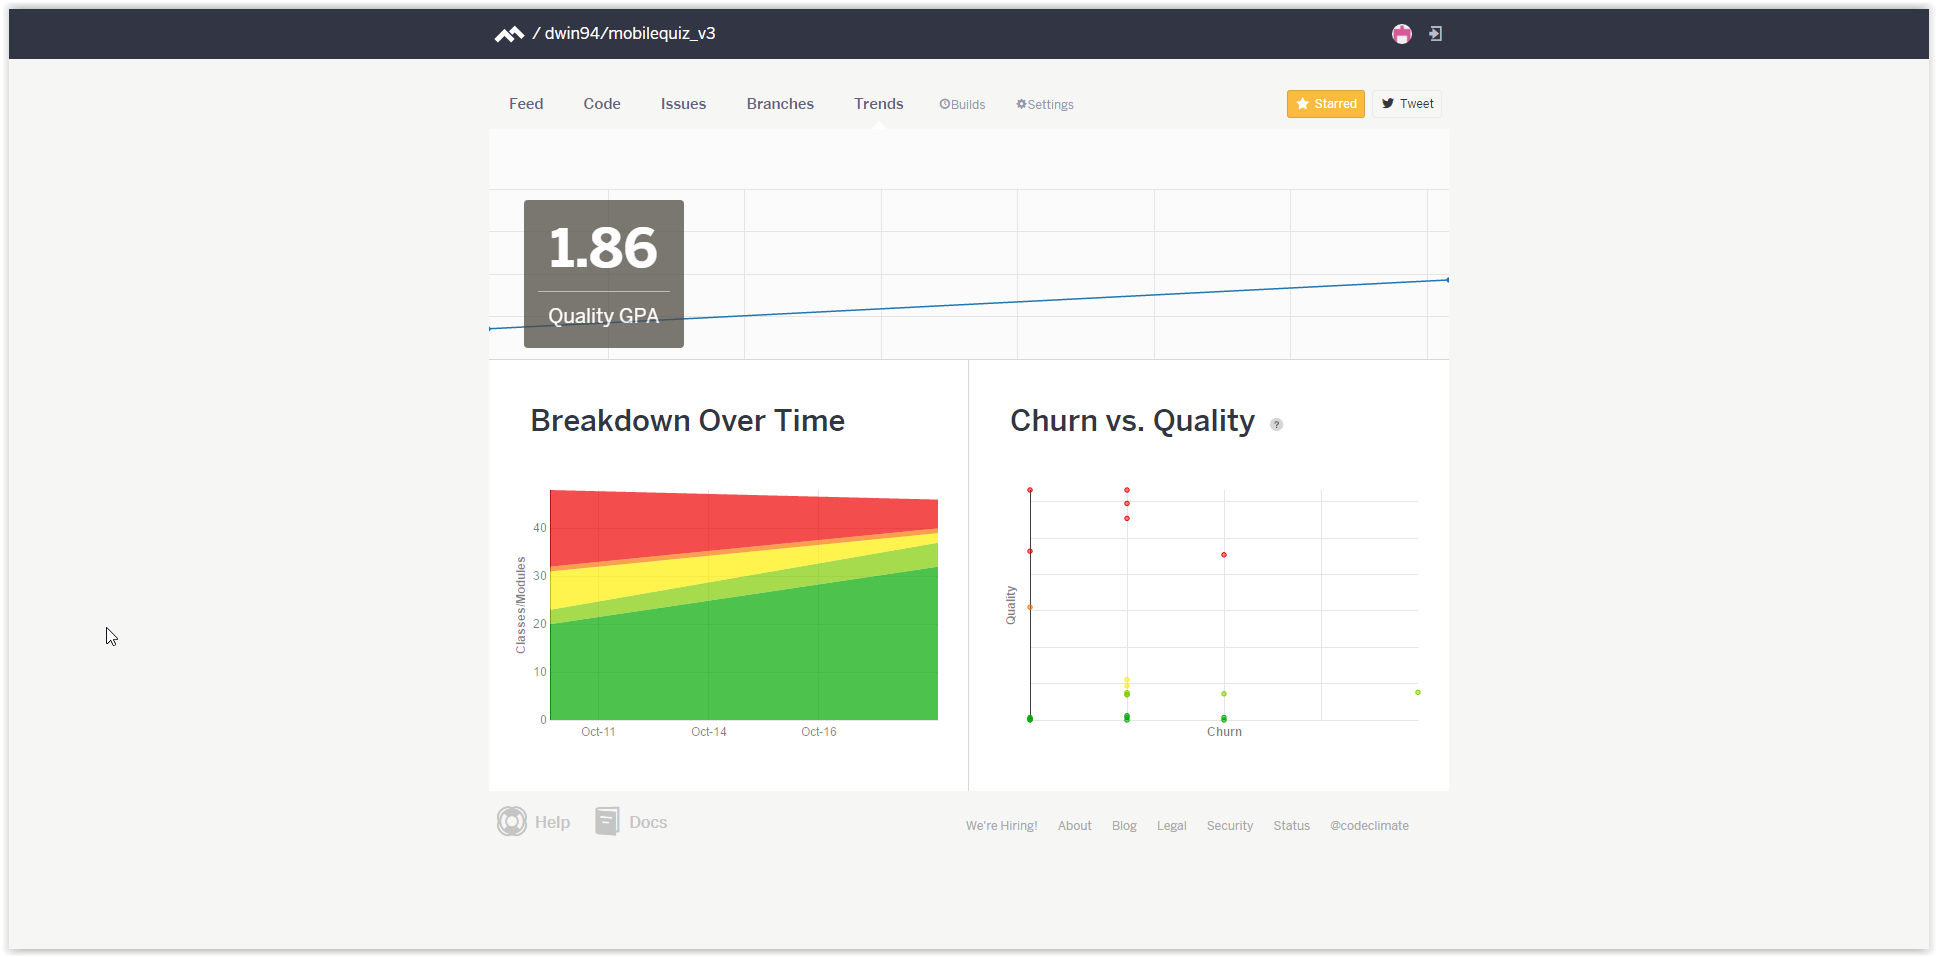
\includegraphics[width=1\textwidth
	]{Images/Stand_Beginn_181016.PNG}
	\caption{Code Climate Stand 18.10.2016 - nach der Verfeinerung der Regeln}
	\cite{codeclimate.com}
\end{figure}


\section{Systemtests mit Selenium}
%automatisierte Systemtests mit Selenium
Selenium IDE ist ein Firefox AddOn für Web-\acrfull{UI}-Tests. Es ermöglicht das Aufnehmen, die Bearbeitung, das Debuggen und das Abspielen von Tests. 

Mit der Hilfe dieses Tools können einfach \gls{User Interface} Tests durchgeführt werden.

\subsection{Methoden}
%Konkretes Vorgehen beschreiben
Mit dem Firefox Plugin von Selenium können die Abläufe die getestet werden sollen einfach aufgenommen werden. Das heisst der Benutzer spielt den korrekten Ablauf durch. Das einzige was von Hand gemacht werden muss, ist das assert-Statement, also die Prüfung, ob der Test korrekt durchgelaufen ist.

Alle erfassten Tests werden abgespeichert und können danach einfach abgespielt werden.


\section{Unit-Tests}
Unit-Tests sind dazu da, einzelne Funktionen zu testen. Wenn eine Basis von Unit-Test bestehen, welche die Funktionalität des Codes abdecken, sind Code-\gls{Refactoring}s leichter umzusetzen. Funktionieren Tests nach dem Umstellen des Codes nicht mehr, so können die Fehler leichter gefunden werden, da die Tests jeweils nur einen kleinen Code-Bereich prüfen.

Zu Beginn war geplant, Unit-Tests mit PHPUnit \cite{phpunit} umgesetzen. Es wäre möglich gewesen, diese Test bei jedem \gls{Commit} automatisch vom Continuous Integration Server Travis CI \cite{travisCI}, ausführen zu lassen. So wäre bei jedem \gls{Commit} überprüft worden, ob noch alles funktioniert.

Das Problem war, dass der Code in einer nicht-testbaren Form geschrieben war und immer noch ist. Die vorhandenen PHP-Dateien enthalten alle lange Methoden mit vielen Nebeneffekten auf diverse Variablen oder die Datenbank. Somit war es aus zeitlichen Gründen nicht möglich, denn gesamten Code testbar umzuschreiben und entsprechende Unit-Tests zu implementieren.



\section{Continuous Integration}
\acrfull{CI} ist ein Prozess, bei dem die einzelnen Software-Komponenten nach dem \gls{Commit} automatisch getestet und anschliessend mit den anderen Komponenten zusammengefügt werden. Dies bringt den Vorteil, dass die Integration der Komponenten laufend geprüft wird und die Unit-Tests Fehler sofort erkennen. Zudem kann die Code-Qualität anhand von verschiedenen Kennzahlen regelmässig gemessen werden.


\begin{figure}[H]
	\centering
	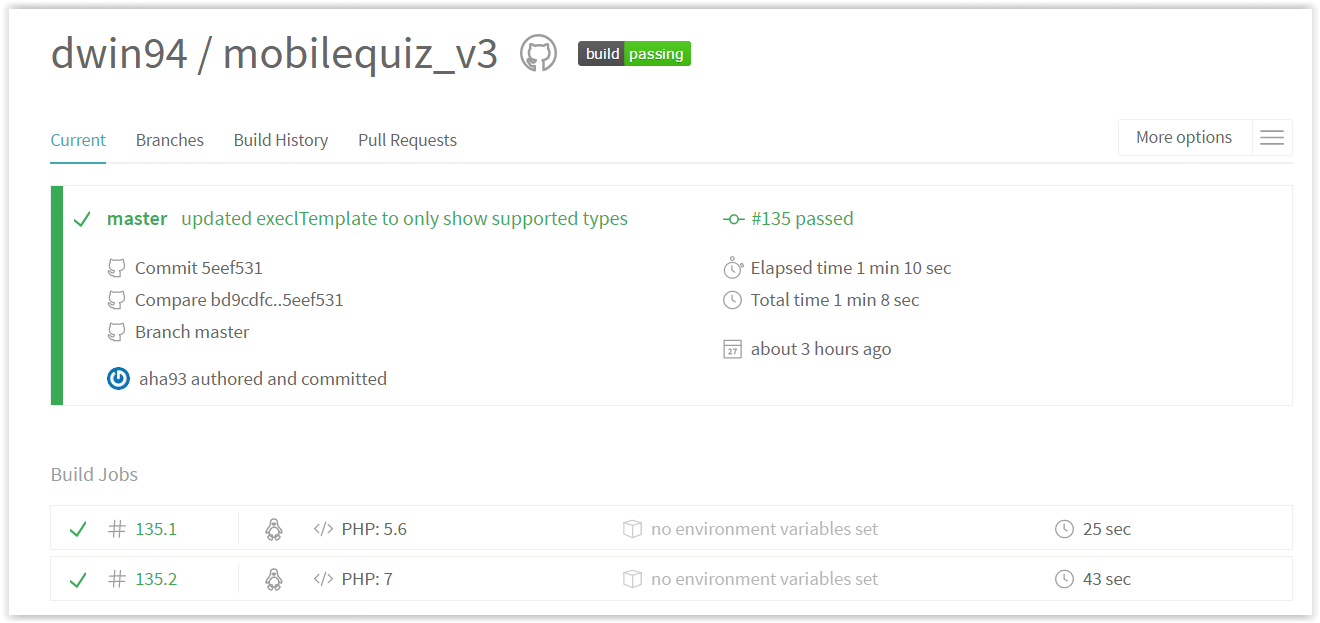
\includegraphics[width=1\textwidth]{Images/travisCI.PNG}
	\caption{TravisCI-Ansicht des letzten Commits}
	\cite{travisCI}
\end{figure}


Dies wurde mit Travis CI \cite{travisCI} teilweise umgesetzt. Unit-Tests waren zwar nicht vorhanden, jedoch prüfte der \acrshort{CI}-Server jeweils die Abhängigkeiten der PHP-Files. Bei erfolgreichem Durchlaufen stiess er zudem das Codestatistik-Tool Code Climate \cite{codeclimate} an, welches anhand von vordefinierten Tests die Code-Qualität mass.
